\documentclass[9pt]{article}

\usepackage[utf8]{inputenc}
\usepackage{geometry}
\geometry{
    a4paper,
    total={170mm,257mm},
    left=15mm,
    right=15mm,
    top=20mm,
    bottom=20mm,
}
\usepackage{multicol}
\usepackage[font=small,labelfont=bf]{caption}
\setlength{\columnsep}{0.25cm}
\usepackage[inline]{enumitem}
\usepackage{amssymb}
\usepackage{xcolor}
\usepackage{mathtools} 
\setlength{\parindent}{0em}
\setlength{\parsep}{0em}
\usepackage{tikz}
\setlength{\parskip}{0em}
\usetikzlibrary{decorations.pathmorphing,patterns}
\usepackage[american,cuteinductors]{circuitikz}
\usetikzlibrary{shapes,arrows,circuits,calc,babel}
% Definition of blocks:
\tikzset{%
  block/.style    = {draw, thick, rectangle, minimum height = 3em,
    minimum width = 3em},
  sum/.style      = {draw, circle, node distance = 2cm}, % Adder
  input/.style    = {coordinate}, % Input
  output/.style   = {coordinate} % Output
}
% Defining string as labels of certain blocks.
\newcommand{\suma}{\Large$+$}
\newcommand{\inte}{$\displaystyle \int$}
\newcommand{\derv}{\huge$\frac{d}{dt}$}

\def\mf{\ensuremath\mathbf}
\def\mb{\ensuremath\mathbb}
\def\mc{\ensuremath\mathcal}
\def\lp{\ensuremath\left(}
\def\rp{\ensuremath\right)}
\def\lv{\ensuremath\left\lvert}
\def\rv{\ensuremath\right\rvert}
\def\lV{\ensuremath\left\lVert}
\def\rV{\ensuremath\right\rVert}
\def\lc{\ensuremath\left\{}
\def\rc{\ensuremath\right\}}
\def\ls{\ensuremath\left[}
\def\rs{\ensuremath\right]}
\def\bmx{\ensuremath\begin{bmatrix*}[r]}
\def\emx{\ensuremath\end{bmatrix*}}
\def\bmxc{\ensuremath\begin{bmatrix*}[c]}
\def\emxc{\ensuremath\end{bmatrix*}}
% \def\t{\lp t\rp}
% \def\k{\ls k\rs}

\newcommand{\demoex}[2]{\onslide<#1->\begin{color}{black!60} #2 \end{color}}
\newcommand{\demoexc}[3]{\onslide<#1->\begin{color}{#2} #3 \end{color}}
\newcommand{\anim}[3]{\onslide<#1->{\begin{color}{#2!60} #3 \end{color}}}
\newcommand{\ct}[1]{\lp #1\rp}
\newcommand{\dt}[1]{\ls #1\rs}

\renewcommand{\familydefault}{\sfdefault}

\begin{document}
\begin{center}
\begin{Large}
\textbf{Linear Systems: Single Input Single Output View Assignment}
\end{Large}
\end{center}
\vspace{0.2cm}

\begin{multicols}{2}
\begin{enumerate}[resume]
    \item Write down the differential equation representing relationship between the loop current $y\ct{t}$ and the input voltage $v\ct{t}$. Assume a initial loop current of $y\ct{0^-} = y_0$.
    \begin{center}
        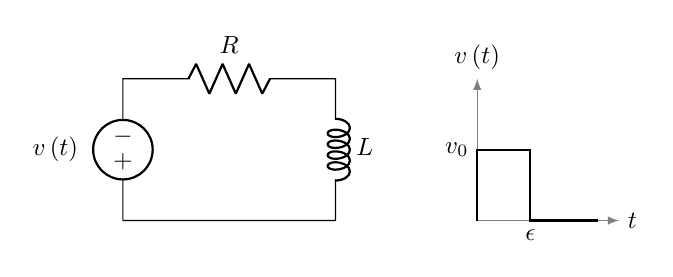
\begin{tikzpicture}[scale=0.9, transform shape]
        \path (0,0) coordinate (ref_gnd);
        \draw
          (ref_gnd) to[american voltage source=$v\lp t\rp$] ++(0,2)
                    to[R=\(R\)] ++(3,0) 
                    to[L=\(L\)] ++(0,-2) 
          -- (ref_gnd);
        
        \draw[-latex, gray] (5, 0) -- (7, 0) node[black, right] {$t$};
        \draw[-latex, gray] (5, 0) -- (5, 2) node[black, above] {$v\ct{t}$};
        \draw[-, black, thick] (5, 0) -- (5, 1) -- (5.75, 1) -- (5.75, 0) -- (6.7, 0);
        \node[black, left] at (5, 1) {$v_0$};
        \node[black, below] at (5.75, 0) {$\epsilon$};
        \end{tikzpicture}
    \end{center}
    \begin{enumerate}
        \item Find the response of the system for the input $v\ct{\bullet}, \forall t \geq 0$ shown in the figure.
        \item Show that for a suitable choice $\epsilon$, $y\ct{t} = 0, \,\, \forall t > \epsilon$.
        \item Assuming $y\ct{0^-} = 0$, what happens to $y\ct{t}$ when, $\epsilon \to 0$ and $v_0 \to \frac{1}{\epsilon}$? Derive the mathematical expression applying this limit. Compare this solution to the input $v\ct{t} = \delta\ct{t}$.
        \item What will happen when $\epsilon \to 0$ and $v_0$ is constant?  
    \end{enumerate}

    \item Derive the differential equation governing the following two mechanical systems. The input to both these systems is the force $f\ct{t}$, and the position $x\ct{t}$ is the output; assume the initial conditions to $x\ct{0^-}, \dot{x}\ct{0^-}$.

    \begin{center}
    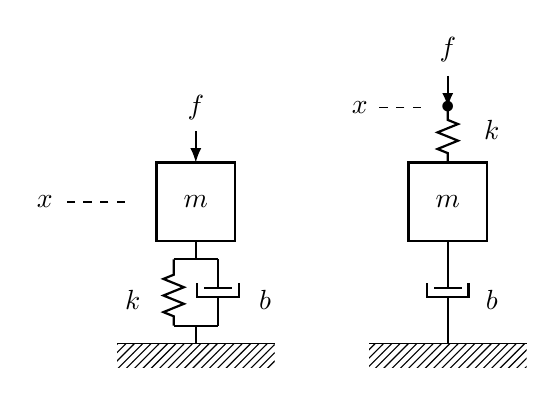
\begin{tikzpicture}[every node/.style={draw,outer sep=0pt,thick}, scale=0.8]
    %define the spring
    \tikzstyle{spring}=[thick,decorate,decoration={zigzag,pre length=0.12cm,post length=0.12cm,amplitude=1.3mm,segment length=6}]

    %define the dashpot
    \tikzstyle{damper}=[thick,decoration={markings,
      mark connection node=dmp,
      mark=at position 0.5 with 
      {
          \node (dmp) [thick,inner sep=0pt,transform shape,rotate=-90,minimum width=15pt,minimum height=3pt,draw=none] {};    
          \draw [thick] ($(dmp.north east)+(2pt,0)$) -- (dmp.south east) -- (dmp.south west) -- ($(dmp.north west)+(2pt,0)$);
          \draw [thick] ($(dmp.north)+(0,-5pt)$) -- ($(dmp.north)+(0,5pt)$);
      }
    }, decorate]

    %define the spring-dashpot
    \tikzstyle{spr-dash}=[thick,decorate,decoration={markings,
      mark connection node=sqr,
      mark=at position 0.5 with
      {
          \node (sqr) [thick,minimum width=16pt,minimum height=24pt,draw=none] {};
          \draw [thick] (sqr.north west) -- (sqr.north east);
          \draw [thick] (sqr.south west) -- (sqr.south east);
          \draw [spring] (sqr.south west) -- (sqr.north west);
          \draw [damper] (sqr.south east) -- (sqr.north east);
      }
      }]

    %define the ground
    \tikzstyle{ground}=[fill,pattern=north east lines,draw=none, minimum width=0.75cm, minimum height=0.3cm]

    %define node stype
    \tikzset{simplenode/.append style={draw=none}}

    \begin{scope}[xshift=0.0cm]
    %draw the frame mass
    \node (M1) [minimum width=1cm,minimum height=1cm] {$m$};
    
    \node (ground-medium) at (M1.south) [ground,yshift=-1.3cm,minimum width=2cm,anchor=north] {};
    \draw (ground-medium.north west) -- (ground-medium.north east);

    \draw [spr-dash] (ground-medium.north) -- (M1.south);
    \node [draw=none] at ($(ground-medium.north)+(-1cm,0.7cm)$) {$k$};
    \node [draw=none] at ($(ground-medium.north)+(1.1cm,0.7cm)$) {$b$};

    \draw [dashed,thin] (M1.west) ++ (-0.5cm, 0) -- +(-1.0cm, 0);
    \node [draw=none, left] at ($(M1.west) + (-1.5cm, 0cm)$) {$x$};

    \draw [-latex,thick] (M1.north) ++ (0, 0.5cm) -- (M1.north);
    \node [draw=none, yshift=0.7cm] at (M1.north) {$f$};
    \end{scope}

    \begin{scope}[xshift=4.0cm]
    %draw the frame mass
    \node (M1) [minimum width=1cm,minimum height=1cm] {$m$};
    \node (ground-medium) at (M1.south) [ground,yshift=-1.3cm,minimum width=2cm,anchor=north] {};
    \draw (ground-medium.north west) -- (ground-medium.north east);

    \draw [damper] (ground-medium.north) -- (M1.south);
    \draw [spring] (M1.north) -- (0, 1.5cm);
    \node [draw=none] at ($(ground-medium.north)+(0.7cm,3.4cm)$) {$k$};
    \node [draw=none] at ($(ground-medium.north)+(0.7cm,0.7cm)$) {$b$};

    \draw [dashed,thin] (M1.west) ++ (0.2cm, 1.5) -- +(-0.75cm, 0);
    \node [draw=none, left] at ($(M1.west) + (-0.5cm, 1.5cm)$) {$x$};

    \draw [-latex,thick] (0, 2.0cm) -- (0, 1.5cm);
    \node[simplenode] at (0, 1.5cm) {$\bullet$};
    \node [draw=none, yshift=0.1cm] at (0, 2.3) {$f$};
    \end{scope}
    \end{tikzpicture}
    \end{center}

    Find the expression for the step response of these two systems. 

    \item Consider a continuous-time LTI system with impulse response, $h\ct{t} = e^{-2t}1\ct{t}$. What is the output of this system to the following inputs using the convolution integral?
    \begin{enumerate*}
        \item $e^{-2t}1\ct{t}$;
        \item $e^{-2t}$;
        \item $e^{-1t}$;
        \item $e^{-4t}$; and 
        \item $\cos\ct{\omega t}$.
    \end{enumerate*}

    Now, obtain the expression for the output of the system for the above inputs using the system's transfer function $H\ct{s}$.

    \item Find the impulse response and transfer functions of the following composition of subsystems with individual impulse response $h_i\ct{t}$.
    \begin{center}
        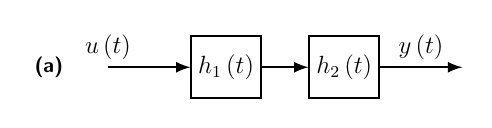
\begin{tikzpicture}[scale=0.75, transform shape, thick, node distance=2cm]
        \draw
            node [input, name=input1] {} 
            node [block, right of=input1] (sys1) {{\large $h_1\ct{t}$}}
            node [block, right of=sys1] (sys2) {{\large $h_2\ct{t}$}}
            node [input, right of=sys2, name=output1] {};
            \draw[-latex] node [above] {{\large $u\ct{t}$}} (input1) -- node {} (sys1);
            \draw[-latex](sys1) -- node {} (sys2);
            \draw[-latex](sys2) -- node[above] {\large $y\ct{t}$} (output1);
            \node[]  at (-1,0) {\textbf{(a)}};
        \end{tikzpicture}

        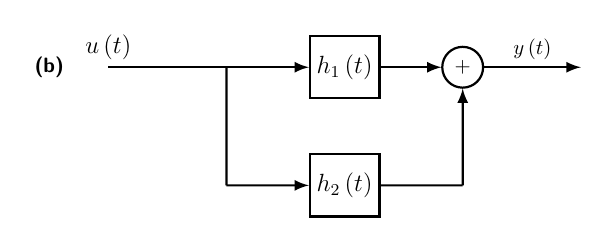
\begin{tikzpicture}[scale=0.75, transform shape, thick, node distance=2cm]
        \draw
            node [input, name=input1] {}
            node [input, right of=input1, name=tempin1] {} 
            node [input, below of=tempin1, name=tempin2] {} 
            node [block, right of=tempin1] (sys1) {{\large $h_1\ct{t}$}}
            node [block, right of=tempin2] (sys2) {{\large $h_2\ct{t}$}}
            node [sum, right of=sys1] (suma1) {$\suma$} 
            node [input, right of=sys2, name=tempout2] {}
            node [input, right of=suma1, name=output1] {};

            \draw[-] node [above] {{\large $u\ct{t}$}} (input1) -- node {} (tempin1);
            \draw[-latex] node {} (tempin1) -- node {} (sys1);
            \draw[-] node {} (tempin1) -- node {} (tempin2);
            \draw[-latex] node {} (tempin2) -- node {} (sys2);
            \draw[-latex](sys1) -- (suma1);
            \draw[-] node {} (sys2) -- node {} (tempout2);
            \draw[-latex] node {} (tempout2) -- node {} (suma1);
            \draw[-latex] node {} (suma1) -- node[above] {$y\ct{t}$} (output1);
            \node[]  at (-1,0) {\textbf{(b)}};
        \end{tikzpicture}

        \begin{tikzpicture}[scale=0.75, transform shape, thick, node distance=2cm]
        \draw
            node [input, name=input1] {}
            node [sum, right of=input1] (suma1) {$\suma$} 
            node [input, below of=suma1, name=tempfb] {} 
            node [block, right of=suma1] (sys1) {{\large $h_1\ct{t}$}}
            node [input, right of=sys1, name=tempout1] {}
            node [input, right of=tempout1, name=output1] {}
            node [input, below of=tempout1, name=tempout2] {}
            node [block, below of=sys1] (sys2) {{\large $h_2\ct{t}$}};

            \draw[-latex] node [above] {{\large $u\ct{t}$}} (input1) -- node {} (suma1);
            \draw[-latex] node {} (suma1) -- node {} (sys1);
            \draw[-] node {} (sys1) -- node {} (tempout1);
            \draw[-latex] node {} (tempout1) -- node {} (output1);
            \draw[-] node {} (tempout1) -- node {} (tempout2);
            \draw[-latex] node {} (tempout2) -- node {} (sys2);
            \draw[-] node {} (sys2) -- node {} (tempin2);
            \draw[-latex] node {} (tempin2) -- node {} (suma1);
            \node[]  at (-1,0) {\textbf{(c)}};
        \end{tikzpicture}
    \end{center}

    \item Consider the second order system, $\ddot{y}\ct{t} + 2\zeta\omega_n\dot{y}\ct{t} + \omega_n^2y\ct{t} = u\ct{t}$. Find the impulse response of this system. Plot the impulse response of the system for $\omega_n = 1$ and the following values of the parameter $\zeta$.
    \begin{enumerate*}
        \item $\zeta = \sqrt{2}$;
        \item $\zeta = 1$;
        \item $\zeta = 0.5$;
        \item $\zeta = 0$;
        \item $\zeta = -0.5$; and 
        \item $\zeta = -1.0$;
    \end{enumerate*}
    For each of these parameter values show the location of the poles of the corresponding transfer function.
\end{enumerate}

\end{multicols}
\end{document}